\section{Теоретическая часть}

\subsection{Введение}
Стационарный электрический ток в замкнутой цепи существует благодаря источникам тока, в которых на носители тока действуют сторонние силы. Электродвижущей силой (ЭДС) на участке цепи называется работа сторонней силы по перемещению единичного положительного заряда:
\begin{align} \label{eq:1}
	\mathcal{E}_{12} = \int_{1}^{2} \vec{E}_{\text{ст}} \cdot d\vec{l}.
\end{align}

Под действием сторонних сил происходит разделение зарядов, возникает кулоновское поле. Работа кулоновской силы:
\begin{align} \label{eq:2}
	\varphi_1 - \varphi_2 = \int_{1}^{2} \vec{E}_{\text{кул}} \cdot d\vec{l}.
\end{align}

На любом участке цепи выполняется закон Ома:
\begin{align} \label{eq:3}
	I R_{12} = \varphi_1 - \varphi_2 + \mathcal{E}_{12}.
\end{align}

\subsection{Измерение ЭДС при помощи вольтметра}
\begin{figure}[H]
	\centering
	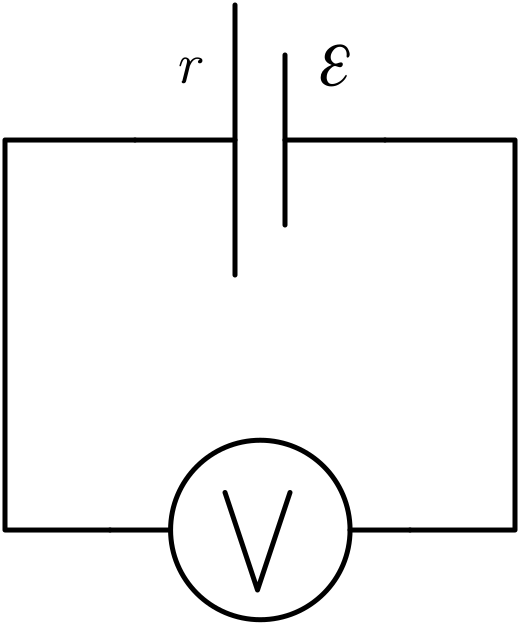
\includegraphics[width=0.3\linewidth]{graph1}
	\caption{Измерение ЭДС при помощи вольтметра.}
	\label{fig:1}
\end{figure}

При подключении вольтметра с сопротивлением $R_v$ к батарее с ЭДС $\mathcal{E}$ и внутренним сопротивлением $r$:
\begin{align} \label{eq:4}
	U = I R_v = \frac{\mathcal{E} R_v}{R_v + r}.
\end{align}

Относительная ошибка измерения:
\begin{align} \label{eq:5}
	\delta\mathcal{E} \approx \frac{r}{R_v}.
\end{align}

\subsection{Метод компенсации}
\begin{figure}[H]
	\centering
	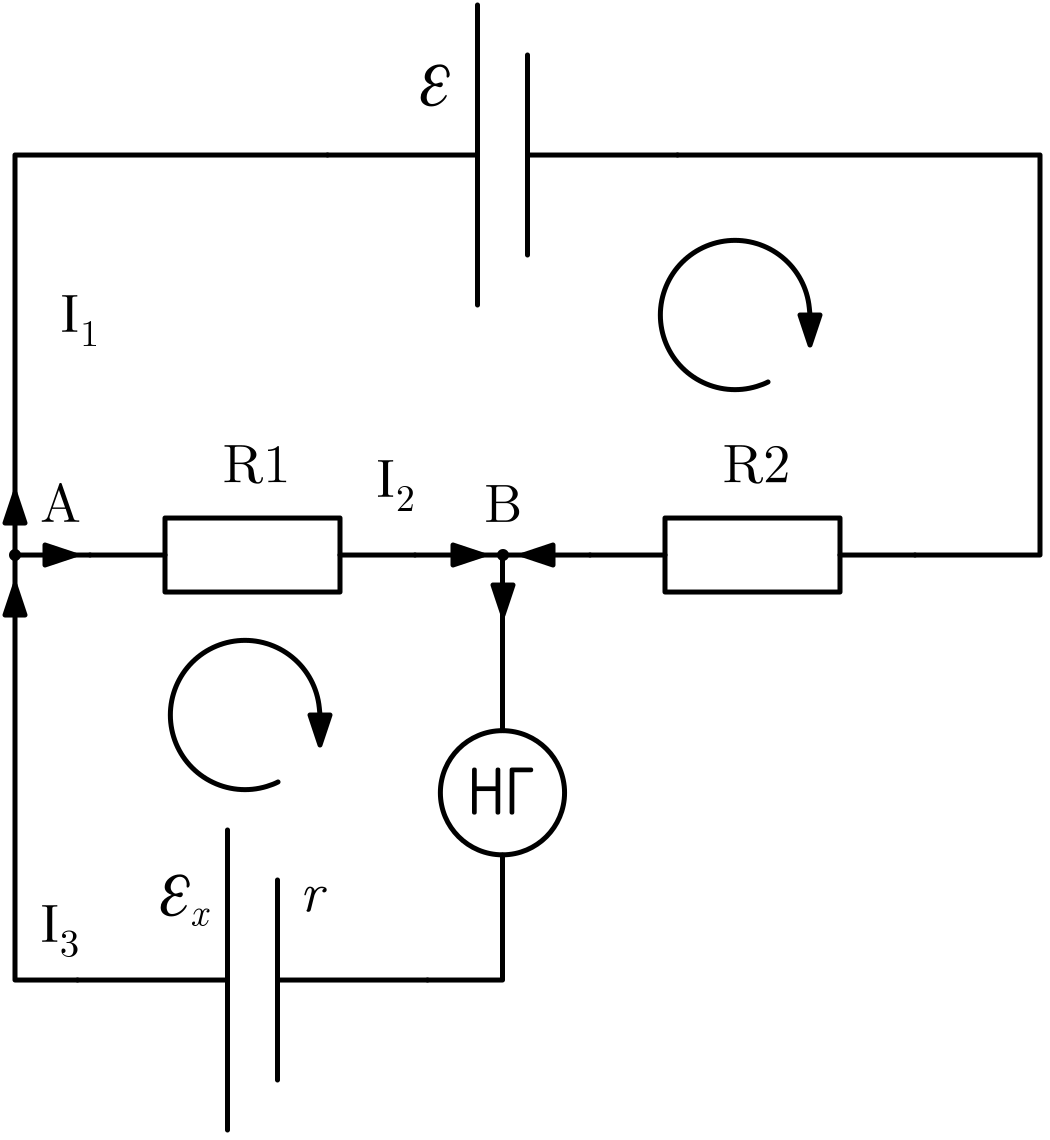
\includegraphics[width=0.7\linewidth]{graph2}
	\caption{Схема измерения ЭДС методом компенсации.}
	\label{fig:2}
\end{figure}

При компенсации ($I_3 = 0$) неизвестная ЭДС:
\begin{align} \label{eq:6}
	\mathcal{E}_x = \frac{R_{1x}}{R} \mathcal{E}.
\end{align}

С использованием эталонной ЭДС:
\begin{align} \label{eq:7}
	\mathcal{E}_x = \frac{R_{1x}}{R_{1N}} \mathcal{E}_N.
\end{align}

\textbf{Вывод формулы для тока через гальванометр:}

По первому закону Кирхгофа:
\[
I_3 = I_1 + I_2.
\]

По второму закону Кирхгофа:
\[
\begin{cases}
	\mathcal{E} = I_1 R_2 - I_2 R_1 \\
	\mathcal{E}_x = I_2 R_1 - I_3 r
\end{cases}
\]

Решая систему, получаем:
\begin{align} \label{eq:8}
	I_3 = \frac{\mathcal{E} R_1 - \mathcal{E}_x R}{rR + R_1 R_2}.
\end{align}

\subsection{Экспериментальная установка}
\begin{figure}[H]
	\centering
	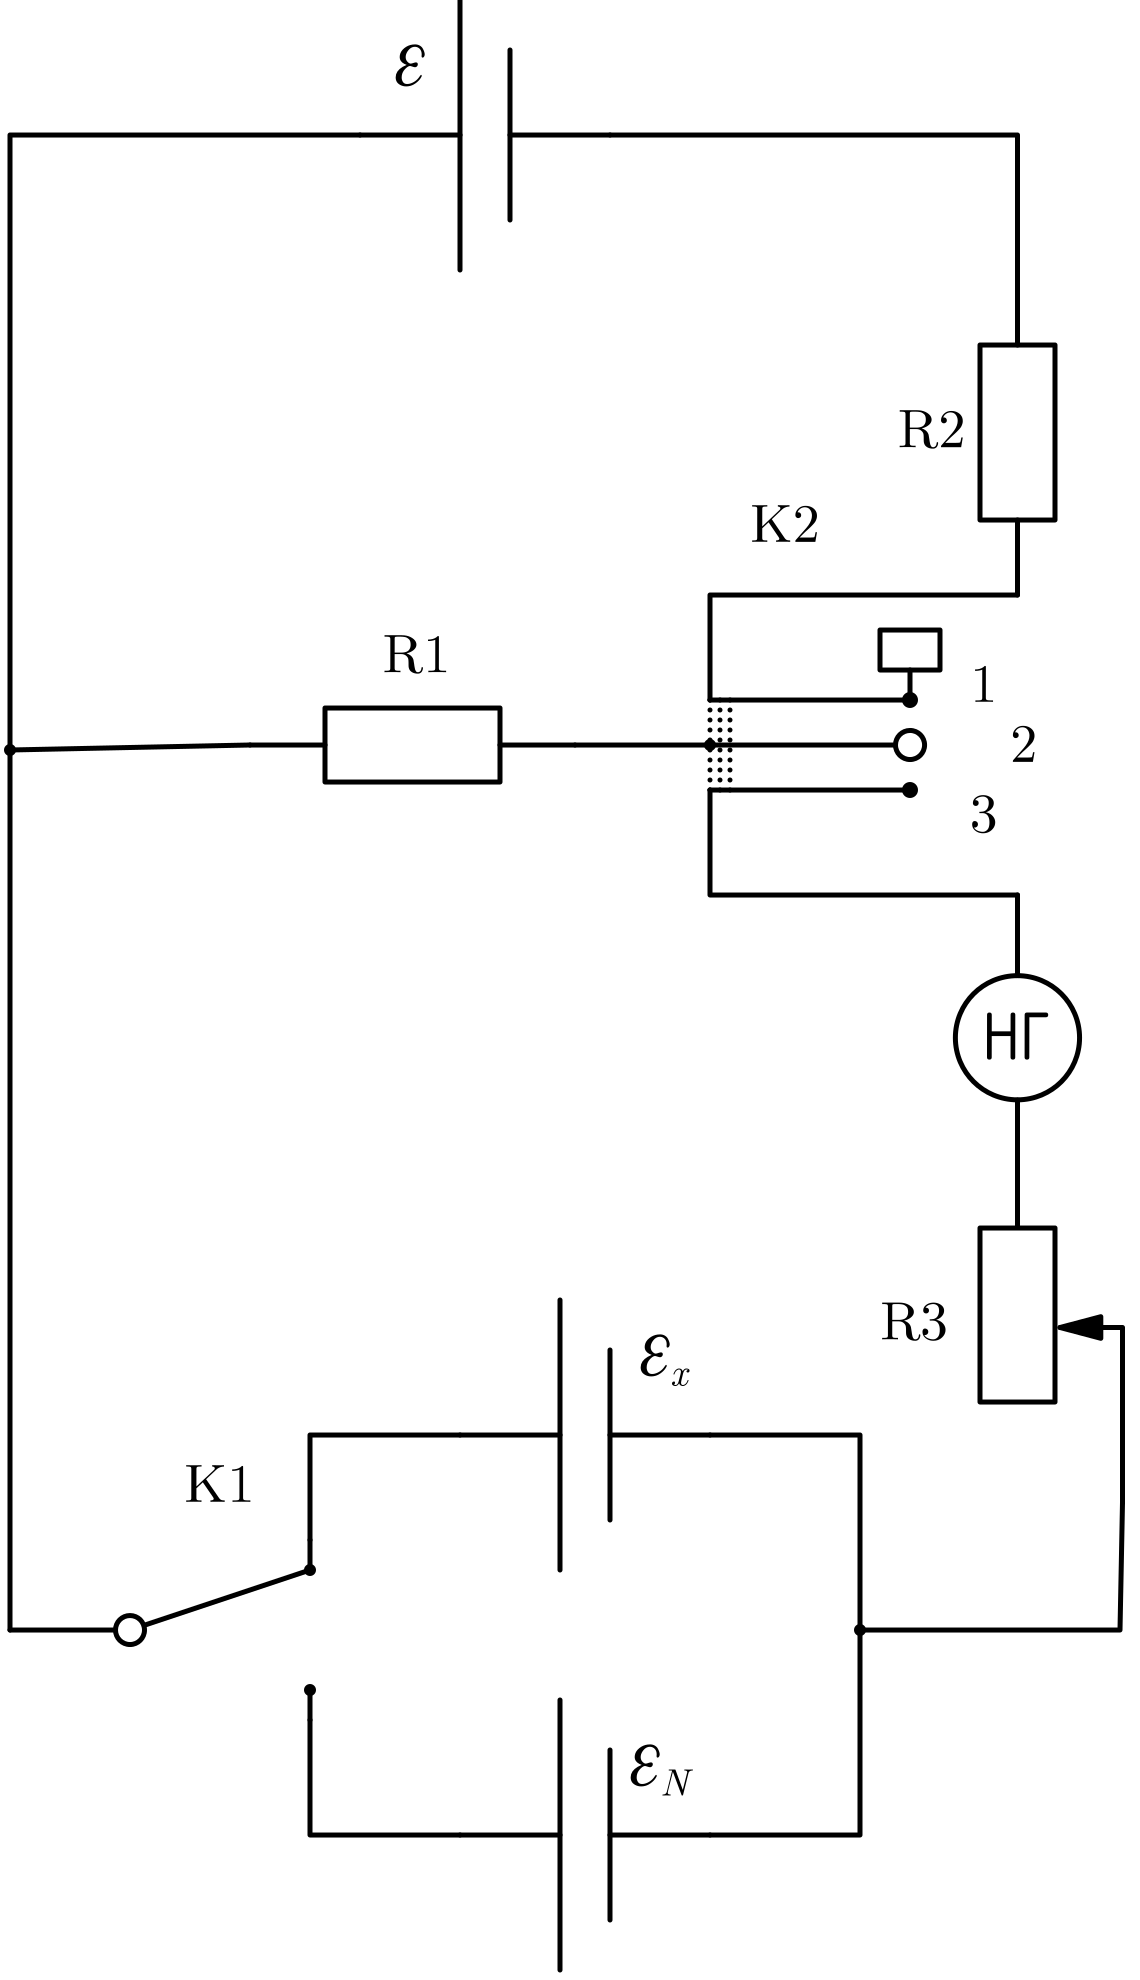
\includegraphics[width=0.7\linewidth]{graph3}
	\caption{Рабочая схема для определения ЭДС}
	\label{fig:3}
\end{figure}

$R_1$ и $R_2$ - штепсельные магазины с $R_1 + R_2 = R = \text{const}$. $R_3$ - защитный резистор.